\documentclass[border=4pt]{standalone}
\usepackage{tikz}
\usetikzlibrary{matrix, positioning, calc}
\begin{document}
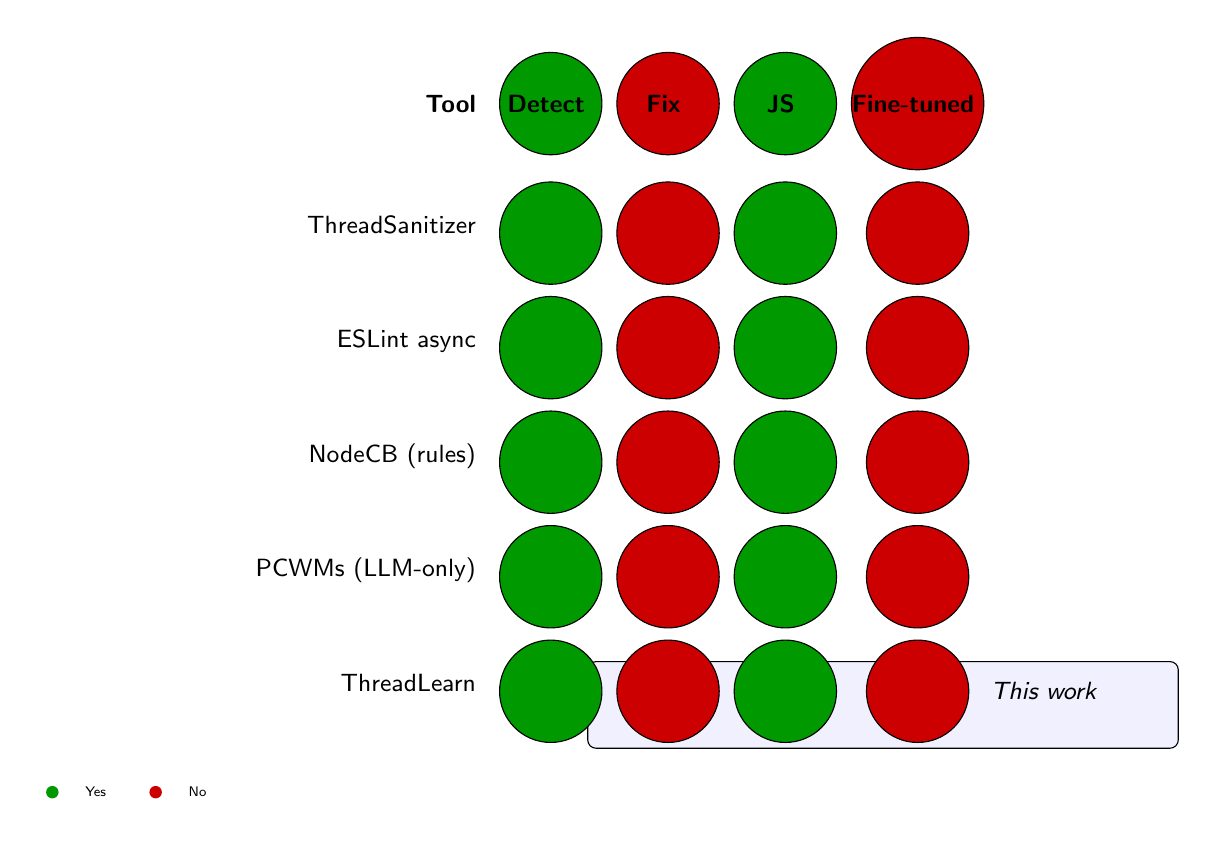
\begin{tikzpicture}[
  cell/.style={minimum width=1.3cm, minimum height=1.4em, font=\small\sffamily, align=center},
  rowhead/.style={text width=4.2cm, align=right, font=\small\sffamily, minimum height=1.4em},
  colhead/.style={font=\small\sffamily\bfseries, minimum height=1.4em},
  chk/.style={circle, fill=green!60!black, minimum size=4.5pt, inner sep=0pt},
  cros/.style={circle, fill=red!80!black, minimum size=4.5pt, inner sep=0pt},
  chkcell/.style={cell, nodes={chk}},
  croscell/.style={cell, nodes={cros}},
]

% Background highlight for ThreadLearn
\draw[fill=blue!6, rounded corners=3pt] (0.35,-4.55) rectangle (7.85,-3.45);

\matrix (m) [matrix of nodes,
  nodes={cell},
  column sep=5pt,
  row sep=4pt,
  row 1/.style={nodes={colhead}},
  column 1/.style={nodes={rowhead}},
  nodes in empty cells,
  column 2/.style={nodes={draw,chk,croscell}},
  column 3/.style={nodes={draw,cros,croscell}},
  column 4/.style={nodes={draw,chk,croscell}},
  column 5/.style={nodes={draw,cros,croscell}},
] {
  Tool & Detect & Fix & JS & Fine-tuned \\
  ThreadSanitizer & & & & \\
  ESLint async & & & & \\
  NodeCB (rules) & & & & \\
  PCWMs (LLM-only) & & & & \\
  ThreadLearn & & & & \\
};

% THIS-WORK label
\node[font=\small\sffamily\itshape, right=0.15cm of m-6-5.east] {This work};

% Legend below
\matrix (leg) [matrix of nodes,
  nodes={font=\tiny\sffamily, anchor=west},
  column sep=3pt,
  row sep=1pt,
] at ($(m.south west)+(0,-0.5)$) {
  \tikz{\node[chk]{};} & Yes & \hspace{6pt}\tikz{\node[cros]{};} & No \\
};

\end{tikzpicture}
\end{document}
